El diseño \textit{hardware} es otro de los componentes clave de este proyecto. En esta
sección se hablará en particular de qué decisiones se han tomado a la hora de montar
el \textit{hardware}, cómo se han configurado y demás.

Por otra parte, se detallará el tipo de placa que se ha utilizado y qué características
tiene de partida que permiten facilitar el desarrollo del proyecto.

Finalmente, se incluyen detalles de cómo es el proceso de manufacturación de la PCB
así como de imágenes que muestran el resultado final.

\subsection{Selección de la placa}
Antes de desarrollar el \textit{hardware} o siquiera materializar la idea, se dedicó
un tiempo de a documentación para determinar qué productos había en el mercado
que pudiesen servir para el propósito de este proyecto. Se consideraron los
siguientes dispositivos (tabla \ref{tab:devices}):


\begin{landscape}
  \begin{table}[H]
    \centering
    \begin{tabularx}{\linewidth}{|c|P{.11}|P{.2}|P{.25}|P{.44}|}
      \hline
      \textbf{\#} & \textbf{Nombre}                                                              & \textbf{Enlace de compra}                                  & \textbf{Enlace a repositorio}                                & \textbf{Comentarios}                           \\
      \hline
      1           & LILYGO\textsuperscript{\textregistered} TTGO T-SIM7000G                      & \url{https://es.aliexpress.com/item/4000542688096.html}    & \url{https://github.com/Xinyuan-LilyGO/LilyGO-T-SIM7000G}    & La placa más completa. Cuenta con conexión SIM %
      LTE CAT4, alimentación externa mediante batería, módulo GPS y módulo SIM.%
      El precio oscila entre los 38\textasciitilde40 \EUR{}. \textit{Firmware} actualizado con%
      regularidad. Módulo SIM 7000G.                                                                                                                                                                                                                                          \\
      \hline
      2           & LILYGO\textsuperscript{\textregistered} Módulo TTGO SIM7600E-H/SIM7600G-H R2 & \url{https://es.aliexpress.com/item/1005001705250713.html} & \url{https://github.com/Xinyuan-LilyGO/LilyGO-T-SIM7600X}    &                                                %
      Placa bastante completa pero más cara. En características, parece similar a la %
      anterior (1). Tiene dos tomas USB Type-C y cuenta con un módulo SIM 7600G. %
      El firmware parece que hace tiempo que no se actualiza. El precio oscila entre %
      los 55\textasciitilde75\EUR{}.                                                                                                                                                                                                                                               \\
      \hline
      3           & LILYGO\textsuperscript{\textregistered} Módulo inalámbrico TTGO t-call       & \url{https://es.aliexpress.com/item/4000959701330.html}    & \url{https://github.com/Xinyuan-LilyGO/LilyGo-T-Call-SIM800} &                                                %
      Placa bastante limitada en recursos con soporte para tarjetas SIM. A diferencia %
      de las dos anteriores, no incluye soporte para tarjetas SD ni tampoco para módulo %
      GPS de forma nativa, por lo que habría que diseñarlo. Tampoco incluye soporte para %
      batería.
      \newline
      Por otra parte, la banda de la tarjeta SIM parece ir en la banda GSM/2G y %
      permitiría hacer solo llamadas o enviar SMS. El precio se encuentra en torno a %
      los 16\EUR{}. Sin embargo, esta placa no se consideraría una opción válida ya que solo %
      permite hacer llamadas/enviar SMS.                                                                                                                                                                                                                                      \\
      \hline
      4           & LILYGO\textsuperscript{\textregistered} TTGO t-call y SIM800C                & \url{https://es.aliexpress.com/item/4001274909689.html}    & \url{https://github.com/Xinyuan-LilyGO/LilyGo-T-Call-SIM800} &                                                %
      Hermana de la placa anterior con algunas prestaciones más. Aplican los mismos comentarios que en la anterior. El precio oscila en torno a los 16\textasciitilde17 \EUR{}.                                                                                                     \\
      \hline
    \end{tabularx}
    \caption{Lista de los distintos dispositivos que se barajaron durante las primeras fases del proyecto.}
    \label{tab:devices}
  \end{table}
\end{landscape}

De entre todos los elementos que se barajaron, se escogió el primero de ellos. Entre
los motivos principales, se destaca que cumplía a la perfección con los requisitos
técnicos del proyecto, es asequible económicamente hablando, tiene un repositorio de
\textit{firmware} bastante actualizado y con ejemplos y permite el desarrollo usando
el \textit{framework} de Arduino, ampliamente probado y con multitud de opciones.

\subsection{El proceso de diseño}
La primera tarea que se tuvo que realizar fue la de diseñar un esquemático y una
huella para el dispositivo escogido, ya que no contaba con ninguna en la librería
estándar de KiCad (programa usado para el diseño de la placa). Para ello, se usaron
los diversos esquemáticos que se encontraban en el repositorio para, por una parte,
definir el \textit{pinout} del dispositivo; y por otro lado, para definir las
dimensiones físicas de la placa en sí.

Usando los recursos con los que se contaban en la web, se tiene que la placa cuenta
con los siguientes conexionados (figura \ref{fig:pinout}):

\begin{figure}[H]
  \centering
  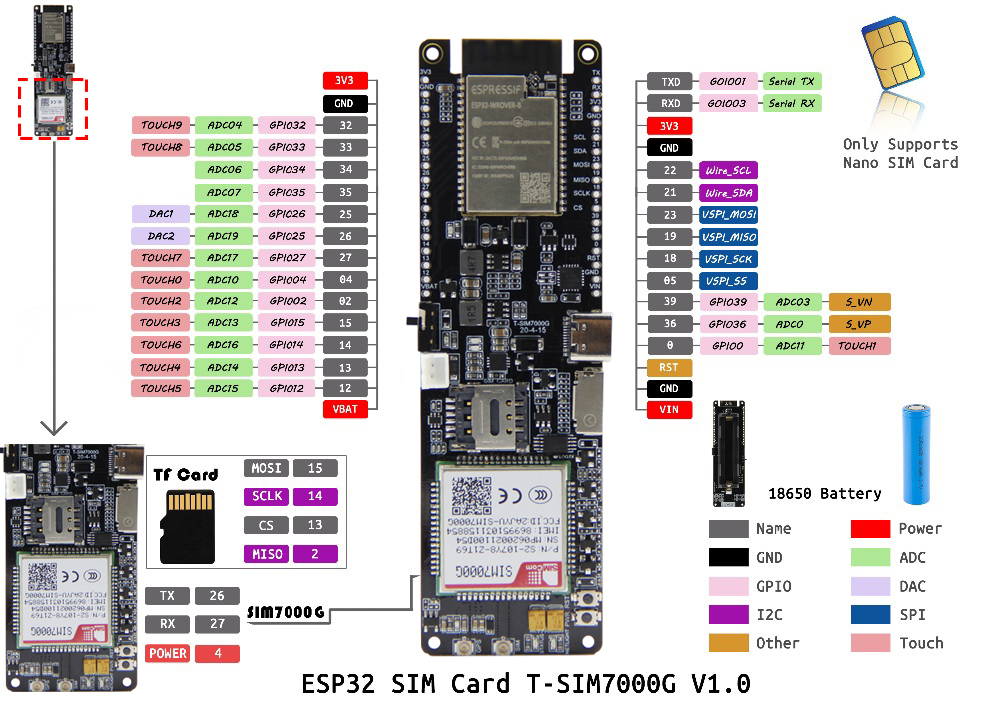
\includegraphics[width=\linewidth]{images/pinout.jpg}
  \caption{Pines y conexiones de la placa \cite{4269LILYGO}.}
  \label{fig:pinout}
\end{figure}

Como se puede apreciar en la figura \ref{fig:pinout}, aunque la interfaz de la
placa provee muchos pines de salida tipo \ac{GPIO} no se pueden usar todos ellos,
ya que algunos están supeditados a otros componentes del sistema (como el módulo SIM).
Según el fabricante, se sabe:

\begin{itemize}
  \item Los pines \texttt{15, 14, 13} y \texttt{2} se usan para la comunicación con
        la tarjeta microSD.
  \item Los pines \texttt{27, 26} y \texttt{4} se usan para el módulo SIM.
\end{itemize}

Es importante tener en cuenta lo anterior para definir qué pines pueden ser utilizados
a la hora de diseñar el producto. De esta manera, el diseño esquemático resultante
para la placa es (figura \ref{fig:tsim-schematic}):

\begin{figure}[H]
  \centering
  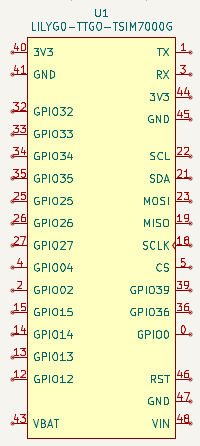
\includegraphics[width=.3\linewidth]{images/TSIM7000G.png}
  \caption{Diseño esquemático del componente T-SIM7000G.}
  \label{fig:tsim-schematic}
\end{figure}

Por otra parte, para la correcta impresión de la placa, es necesario definir también
una huella que se corresponderá con el modelo físico del dispositivo. En este caso,
se usaron los esquemas provistos por el fabricante:

\begin{figure}[H]
  \centering
  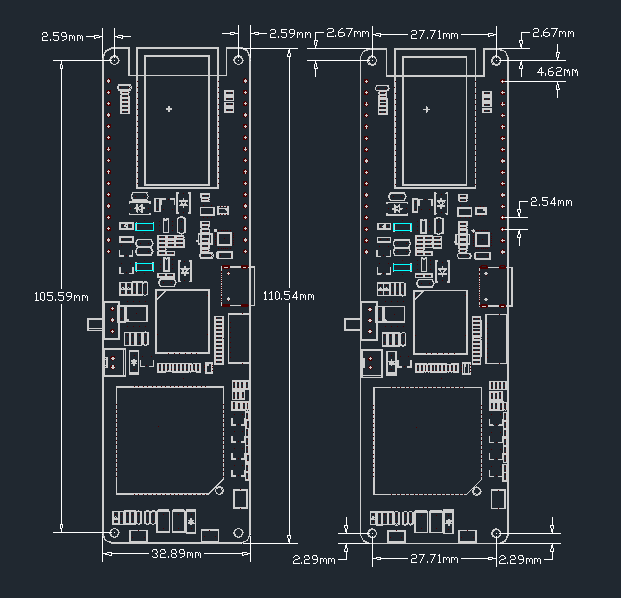
\includegraphics[width=\linewidth]{images/dimensions.png}
  \caption{Dimensiones de la placa T-SIM7000G, según el fabricante \cite{4269LILYGO}.}
  \label{fig:dimensions}
\end{figure}

Usando el editor de huellas de KiCad, se definió la siguiente librería:

\begin{figure}[H]
  \centering
  \begin{minipage}{.4\linewidth}
    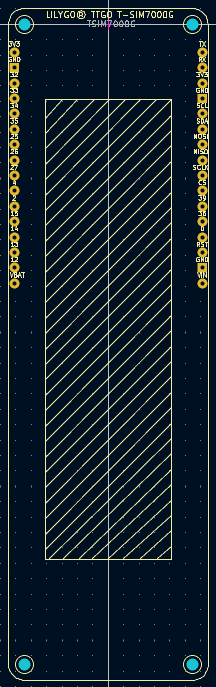
\includegraphics[width=\linewidth]{images/tsim-footprint.png}
    \caption{Huella de la placa T-SIM7000G hecha con KiCad.}
    \label{fig:tsim-footprint}
  \end{minipage}
  \hfill
  \begin{minipage}{.4\linewidth}
    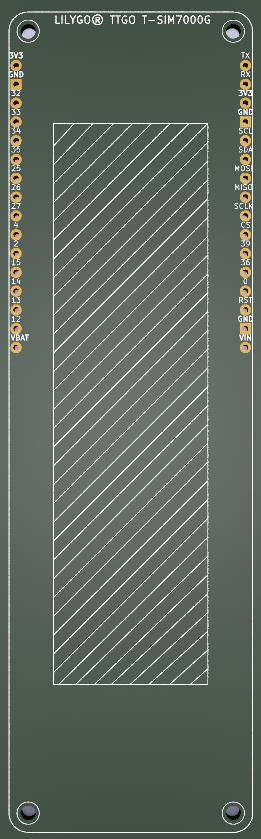
\includegraphics[width=\linewidth]{images/TSIM7000G-3D.png}
    \caption{Visión 3D de la huella para la placa T-SIM7000G.}
    \label{fig:tsim-3d}
  \end{minipage}
\end{figure}

Un factor interesante a destacar es la zona rayada en el interior de la placa. Esta
zona se define así porque se pretende que sea un área de no conexión, ya que puede
ser taladrada. Esto es así porque la placa cuenta con un \textit{slot} para una
batería que va debajo de la misma, ocupando bastante espacio (tanto a lo largo como
a lo alto). Este área se define así para evitar añadir pistas en esa zona por si,
en una etapa posterior de la fabricación, se quiere taladrar para que la batería
quede por debajo.

Esta característica se puede apreciar mejor en la figura \ref{fig:tsim-battery}:

\begin{figure}[H]
  \centering
  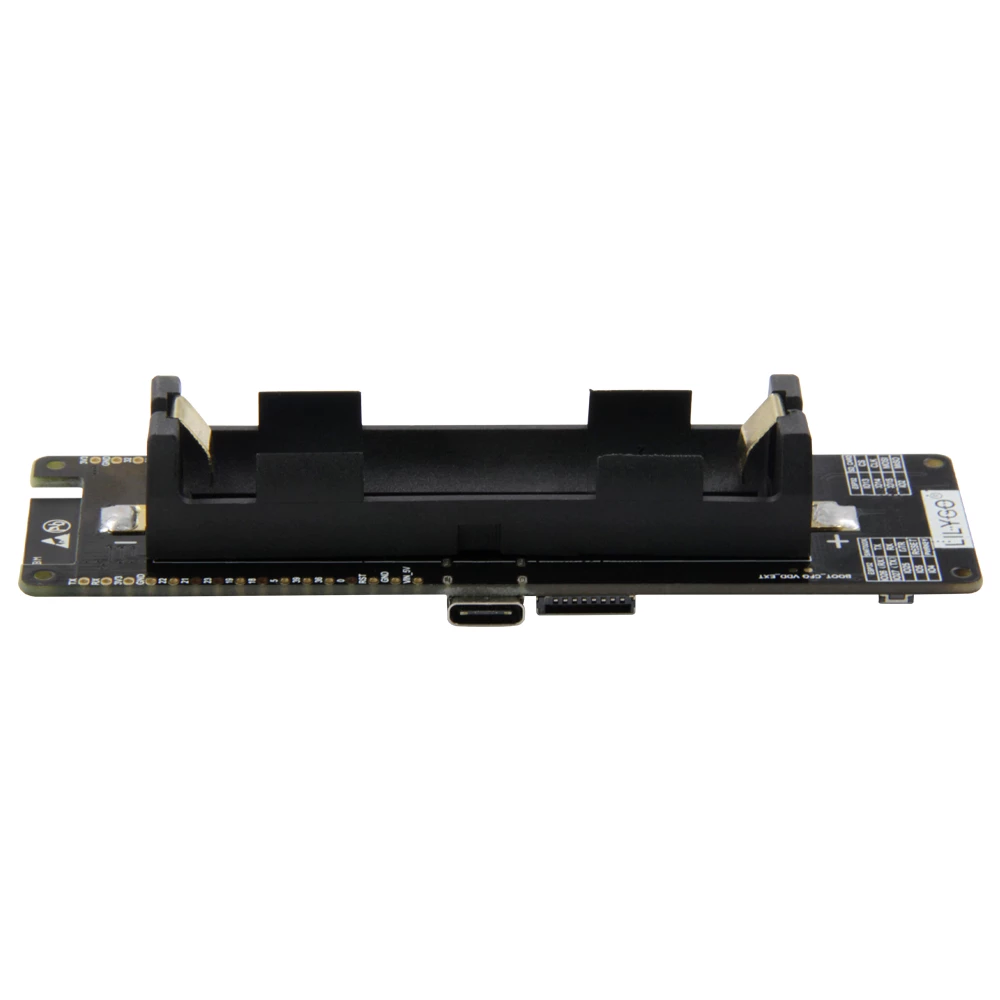
\includegraphics[width=\linewidth]{images/tsim-battery.png}
  \caption{\textit{Slot} para la batería enganchada a la placa T-SIM7000G \cite{4269LILYGO}.}
  \label{fig:tsim-battery}
\end{figure}

Con el dispositivo debidamente verificado, se puede pasar a la siguiente etapa: el
diseño de la PCB. La visión general del sistema se muestra en la figura \ref{fig:general-schematic}:

\begin{figure}[H]
  \centering
  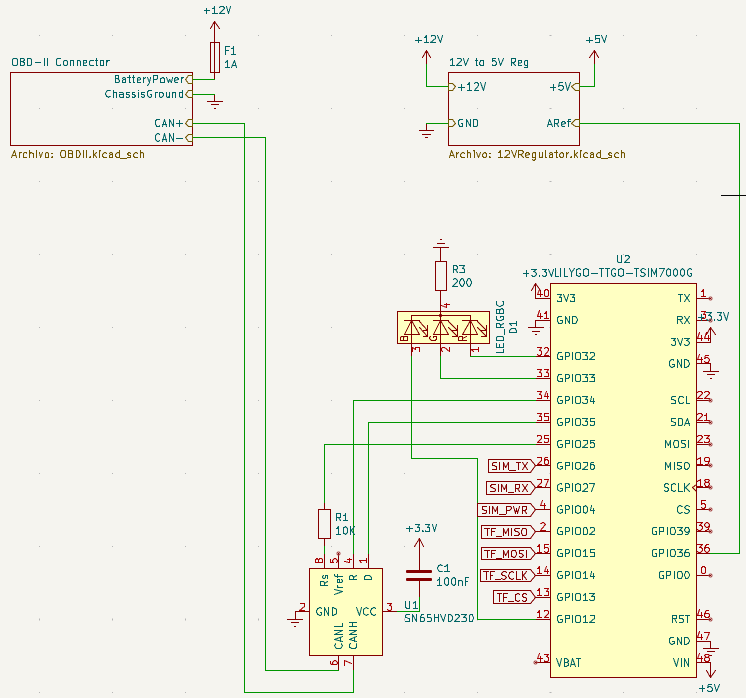
\includegraphics[width=\linewidth]{images/general-schematic.png}
  \caption{Esquemático general que modela el \textit{hardware} del sistema.}
  \label{fig:general-schematic}
\end{figure}

Por simplificar el diseño, el esquemático se divide en tres módulos: conexionado con el
vehículo mediante \ac{OBD}--II, conexionado eléctrico (fuente de alimentación) y la
placa T-SIM7000G con sus periféricos.

\begin{figure}[H]
  \centering
  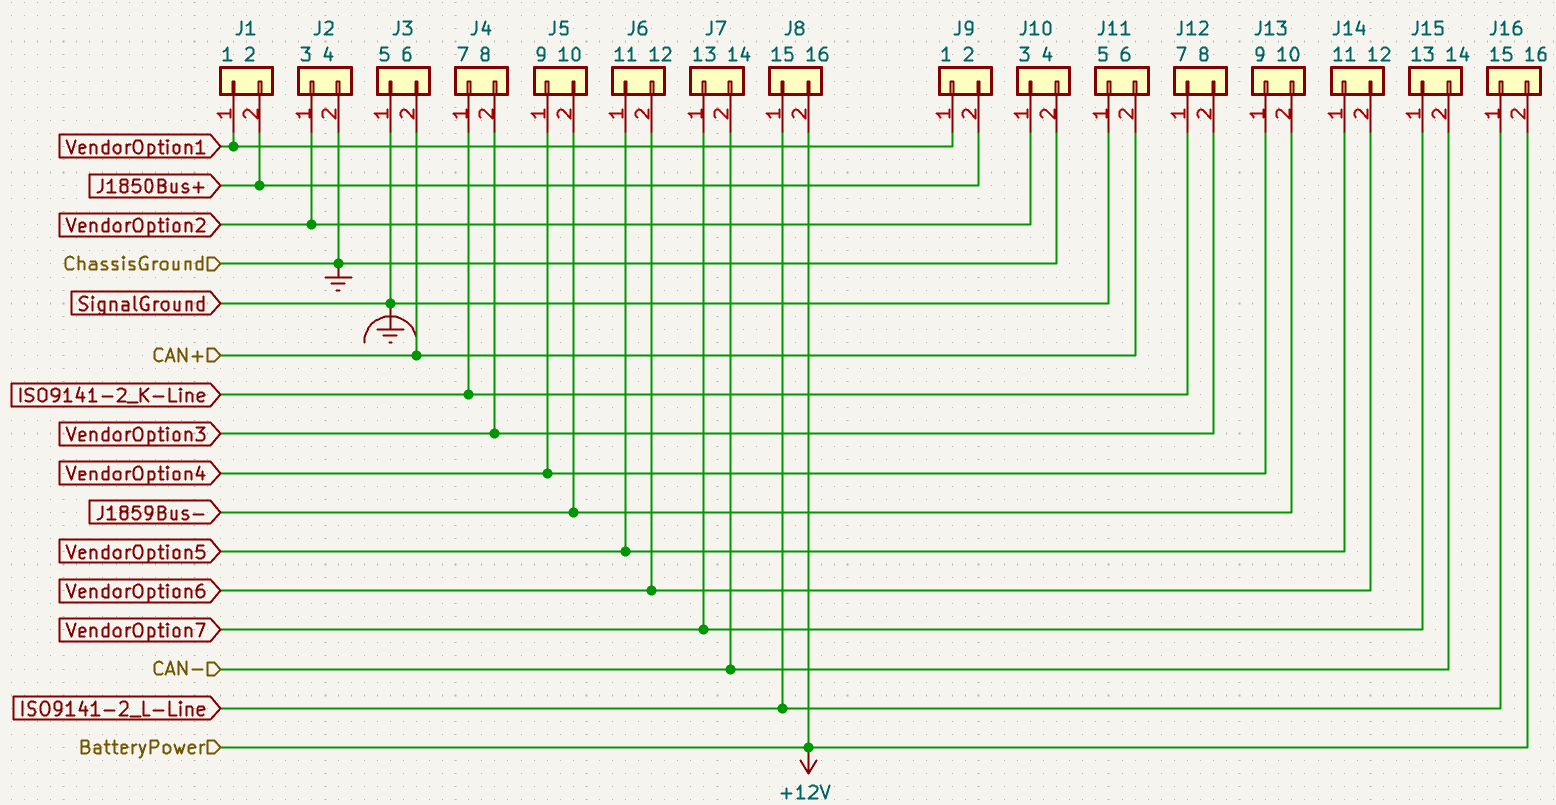
\includegraphics[width=\linewidth]{images/obd-ii-interface.png}
  \caption{Interfaz de comunicaciones de \ac{VIMS} con \ac{OBD}--II.}
  \label{fig:obd-ii-interface}
\end{figure}

En la figura \ref{fig:obd-ii-interface} se muestra la interfaz de comunicaciones
de \ac{VIMS} con el vehículo, mediante \ac{OBD}--II. La estructura puede parecer
un tanto peculiar: 16 conexiones puenteadas entre sí, con unos terminales de entrada
y otros de salida, marcando únicamente 4 conexiones hacia el exterior.

La decisión detrás de este diseño es la de mantener la comunicación con el exterior:
una vez \ac{VIMS} esté conectado con el vehículo, no debe ser necesario quitarlo para
poder conectar otro dispositivo \ac{OBD}--II al vehículo. Por ello, el propio dispositivo
ofrece un terminal de salida en donde otro aparato puede conectarse y acceder a los datos.

En principio, no debería haber problema de pérdidas de los paquetes ya que internamente
se trabaja con el bus \ac{CAN}, que permite que una cantidad arbitraria de nodos se
conecten y lean la información.

De todos los terminales disponibles, \ac{VIMS} solo hace uso de cuatro:

\begin{enumerate}
  \item[\texttt{ChassisGround}] ofrece una conexión de tierra al chasis del vehículo,
    y es la que se debe usar habitualmente para encender el dispositivo. Existe otra
    toma ``\texttt{SignalGround}'' que se usa para depurar errores en la comunicación
    \ac{CAN}, ya que permite conectar un osciloscopio y analizar la onda limpia generada
    por las comunicaciones.
  \item[\texttt{CAN+}] es el valor positivo de la señal \ac{CAN}, que se debe conectar
    al terminal correspondiente para poder interpretar los mensajes recibidos por
    el vehículo.
  \item[\texttt{CAN-}] es el valor negativo de la señal \ac{CAN}, que se debe conectar
    al terminal correspondiente para poder interpretar los mensajes recibidos por
    el vehículo.
  \item[\texttt{BatteryPower}] provee de alimentación directamente desde los bornes de
    la batería, por lo general $12V$ (aunque puede variar según la región).
\end{enumerate}

El resto de elementos están etiquetados para identificar más fácilmente qué líneas
están en uso y facilitar añadir una conexión nueva posteriormente.

\begin{figure}[H]
  \centering
  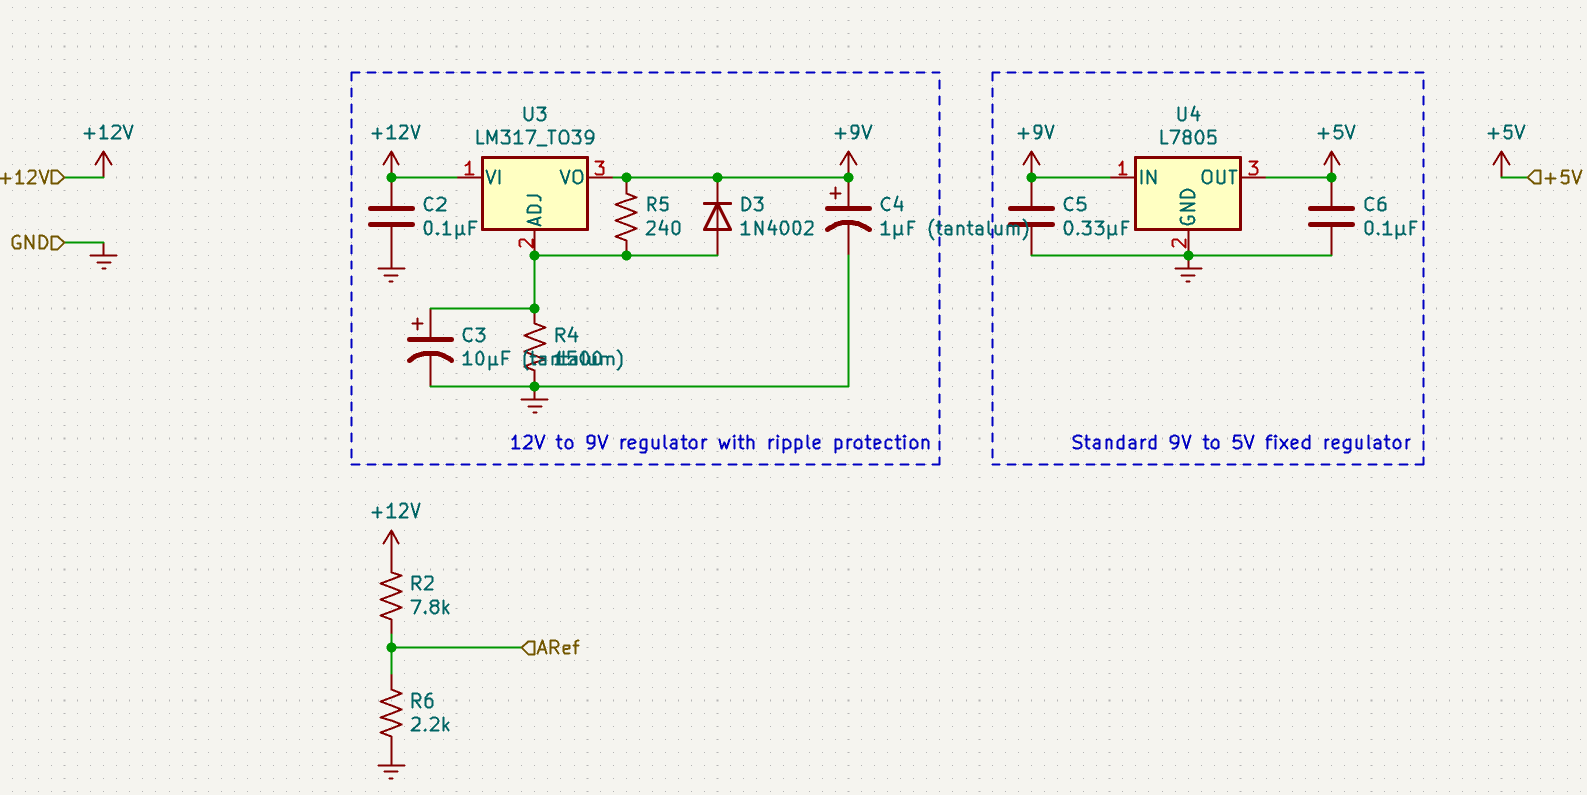
\includegraphics[width=\linewidth]{images/12vregulator.png}
  \caption{Circuito regulador de tensión del dispositivo \ac{VIMS}.}
  \label{fig:12v-regulator}
\end{figure}

En la figura \ref{fig:12v-regulator} se tiene el regulador de tensión del dispositivo
\ac{VIMS}, que toma los $12V$ provistos por la batería del vehículo y los transforma
en un nivel de tensión adecuado para la placa y los componentes que la conforman, en
este caso, $5V$.

El sistema usa dos reguladores de tensión para adecuarla al valor deseado: uno primero
que reduce de $12V$ a $9V$ y el segundo que transforma esos $9V$ en $5V$. Esto se hace
así por un motivo: la disipación de calor. En el caso peor, un dispositivo \ac{VIMS}
puede encontrarse en el interior de un vehículo dándole el sol directo y pudiendo
llegar a alcanzar temperaturas de $60~\tccentigrade$. Definiendo un único regulador
que redujese de $12V \rightarrow 5V$, se tenía que:

\begin{gather*}
  P_{max} = V \cdot I_{max} \\
  P_d = \frac{T_{j_{max}} - T_{amb}}{\theta_{JA}} \\[1ex]
  P_d < P_{max} \Longrightarrow \text{hace falta disipador}
\end{gather*}

Para las características del circuito:

\begin{gather*}
  P_{max} = 7V \cdot 1.2A = 8.4W \\
  P_d = \frac{125 - 60}{15.9} = 4.08W \\
  P_d \le P_{max} \Longrightarrow \text{Hace falta disipador}
\end{gather*}

Sin embargo, introduciendo una doble disipación este problema se mitiga ya que el
primer regulador hace una primera reducción del voltaje y el segundo la restante.

Cabe destacar que el primer regulador sigue un circuito recomendado por el fabricante
que ayuda a reducir el ruido en el pin de ajuste gracias al condensador \texttt{C3}.
El diodo \texttt{D3} se introduce para descargar el condensador \texttt{C3} en caso de
que la salida se conecte a tierra. En este caso, como la corriente de entrada viene
directamente desde la batería o el alternador del vehículo, es posible que haya
bastantes fluctuaciones en la alimentación de entrada y este circuito se ha considerado
fundamental para el desarrollo del sistema eléctrico del dispositivo.

La ecuación de funcionamiento que ofrece el fabricante para este dispositivo es
(ecuación \ref{eq:lm317}):

\begin{equation}\label{eq:lm317}
  V_O = V_{Ref} \cdot \left(1 + \frac{R_2}{R_1}\right) + I_{Adj} \cdot R_2
\end{equation}

De la ecuación anterior, hay que tener en cuenta ciertos datos:

\begin{itemize}
  \item Por construcción, el fabricante establece $V_{Ref} = 1.25V$.
  \item Por construcción, la corriente $I_{Adj}$ tiene un valor pico de $100~\mu A$.
        En este caso no se tiene en consideración por no ser significativo.
\end{itemize}

Por ende, la ecuación que se obtiene para el regulador es (cambiando los nombres de
las resistencias para cuadrar con el circuito diseñado):

\begin{equation*}
  V_O = 1.25V \cdot \left(1 + \frac{R_4}{R_5}\right)
\end{equation*}

Teniendo en cuenta los voltajes requeridos para las etapas de alimentación del
circuito, se ha fijado la resistencia $R_5 = 240\Omega$ (por recomendación del
fabricante) y se obtiene que:

\begin{gather*}
  9V = 1.25V \cdot \left(1 + \frac{R_4}{240\Omega}\right) \\
  \frac{7V}{1.25V} - 1 = \frac{R_4}{240\Omega} \\
  R_4 = 240\Omega \cdot \left(\frac{9V}{1.25V} - 1\right) \\
  R_4 \approx 1488\Omega \Longrightarrow 1500\Omega
\end{gather*}

Con la ecuación anterior se obtiene un voltaje de salida de $9.0625V$, suficiente
para ser introducido en el segundo regulador. Este segundo regulador es el
L7805CV que reduce cualquier tensión superior a $7V$ a $5V$, con el rango óptimo
de operación en torno a los $9V$ de entrada. El fabricante recomienda, para un
modo de funcionamiento de regulación fija de tensión, el siguiente esquemático
(figura \ref{fig:l78}):

\begin{figure}[H]
  \centering
  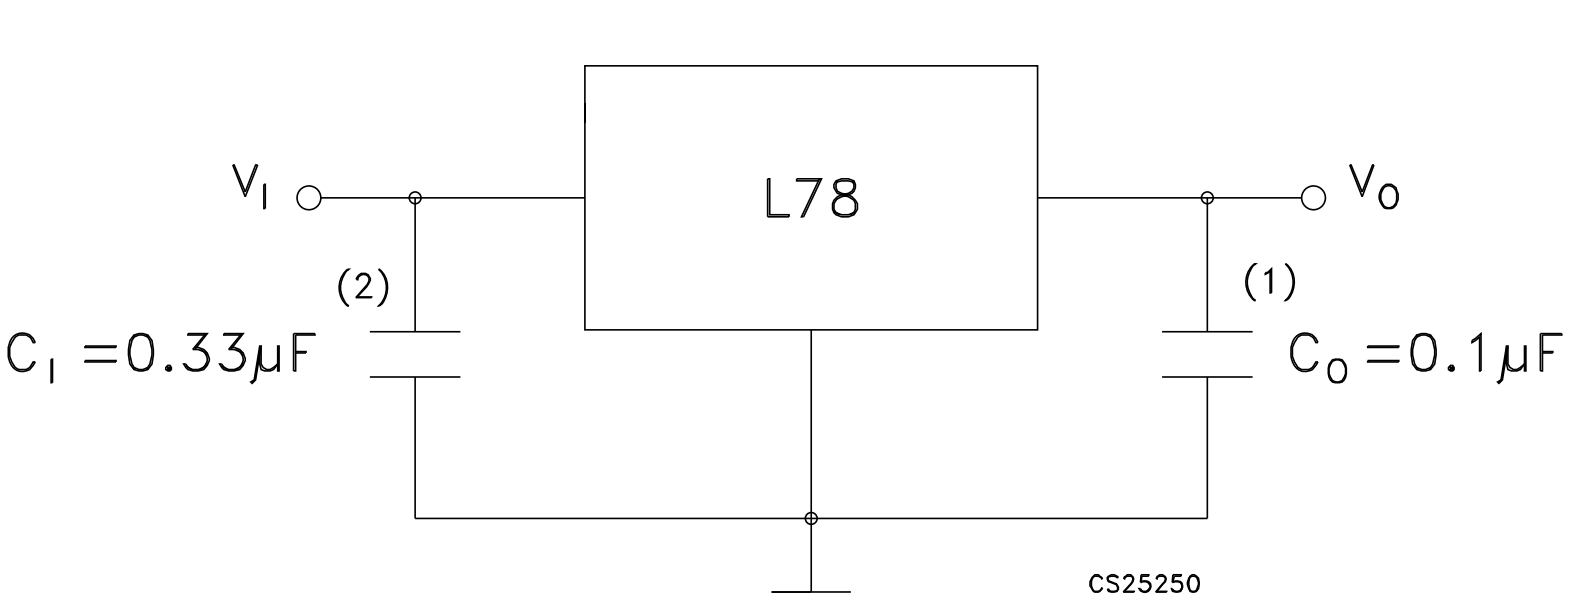
\includegraphics[width=\linewidth]{images/fixed-voltage.png}
  \caption{Circuito regulador de tensión para el L7805CV \cite{L7805CVSTMicroelectronicsMouser}.}
  \label{fig:l78}
\end{figure}

Como se introdujo en el primer salto la protección contra las oscilaciones en la
entrada, este regulador no necesita ninguna configuración más.

El último elemento que se ha introducido en el sistema es el voltaje de referencia
marcado en la salida como ``\texttt{ARef}''. Este pequeño circuito no es más que un
divisor de tensión el cual se usará para saber qué valor de tensión es la que ofrece
el vehículo al que se está conectado. La intención es que ese pin vaya conectado a un
\ac{ADC} de la placa T-SIM7000G y se use dicho convertidor para obtener en digital
el valor equivalente a la corriente de entrada mediante una sencilla operación matemática
conocida como el mapeo.

El divisor de tensión responde ante la siguiente ecuación:

\begin{equation*}
  V_O = V_I \cdot \frac{R_2}{R_1 + R_2}
\end{equation*}

En este circuito, con las resistencias que se utilizan, se tiene:

\begin{equation*}
  V_O = V_I \cdot \frac{2.2K\Omega}{7.8K\Omega + 2.2K\Omega}
\end{equation*}

La idea fundamental detrás de este divisor de tensión es:

\begin{itemize}
  \item Con valores de las resistencias tan elevados, la corriente que circula
        por este circuito es mínima, ya que no interesa tener picos de entrada
        en el dispositivo y se reduce el consumo.
  \item Los vehículos, cuando están ``en frío'' (sin arrancar, parados durante
        cierto tiempo) dan un valor de tensión por debajo de los $12V$ habitualmente,
        signo de que se está alimentando de la batería y que esta se está descargando.
  \item Cuando un vehículo se ha arrancado, entra en funcionamiento el alternador
        que provoca que el sistema se desconecte de la batería y funcione con un
        valor de tensión mayor de lo habitual ($> 12V$) ya que la batería siempre
        se está recargando.
  \item Cuando un vehículo se acaba de aparcar y se ha apagado el motor (ergo se
        ha detenido el alternador), la tensión del sistema cae nuevamente a $12V$
        o superior, pero es una diferencia de tensión de al menos $1.1V$ de media.
        Ese evento se puede detectar fácilmente para identificar que el vehículo se
        ha apagado y que el sistema debe entrar en modo de bajo consumo.
\end{itemize}

Con estas ideas en mente, se puede observar cómo el divisor de tensión anterior está
diseñado para detectar una tensión máxima de $15V$ (asumiendo que $\max\left(V_O\right) = 3.3V$,
que es la tensión con la que funciona la placa):

\begin{equation*}
  3.3V = V_I \cdot \frac{11}{50} \Longrightarrow V_I = 15V
\end{equation*}

Ese valor de entrada en el \ac{ADC} se mapeará a $4096$ (porque el \ac{ADC} tiene
12 bits de resolución) y se puede usar la función matemática de mapeo para obtener
el equivalente valor de entrada:

\begin{equation}\label{eq:map-function}
  V_I = \frac{\left(x - x_{min}\right) \cdot \left(V_I^{max} - V_I^{min}\right)}{x_{max} - x_{min}} + V_I^{min}
\end{equation}

Dicha ecuación quedaría así para los datos de resolución del \ac{ADC}:

\begin{equation*}
  V_I = \frac{15x}{4096}
\end{equation*}

Esto es por los siguientes valores:

\begin{equation*}
  \left\{
  \begin{aligned}
    x_{min}   & = 0~\text{(se acepta no tener tensión de entrada)}  \\
    V_I^{max} & = 15V~\text{(máximo teórico de tensión esperada)}   \\
    V_I^{min} & = 0V~\text{(se acepta no tener tensión de entrada)} \\
    x_{max}   & = 4096~\text{(resolución máxima del \ac{ADC})}
  \end{aligned}
  \right.
\end{equation*}

Finalmente, aunque se encuentra fuera de este segmento del circuito, se incluye un
fusible de $1.5A$ a la entrada de la toma de corriente de la batería del coche
para proteger tanto al sistema como al vehículo en sí. Habitualmente, los automóviles
cuentan con un conjunto de fusibles que protegen ciertos componentes del sistema. Esto
aplica también para el conjunto de componentes del \ac{OBD}--II en la mayoría de las
ocasiones, pero existen vendedores que no protegen dicho puerto con un fusible.

Se estima que los consumos pico de la placa no superen los $0.5A$; sin embargo, el valor
del fusible se pone tan elevado en comparación porque es difícil encontrar de menor
intensidad en el mercado y porque sirve únicamente para detección de cortos y aislamiento
del sistema.

Ya por último queda el bloque de la placa T-SIM7000G, que aúna las conexiones del sistema
y subsistemas. El componente principal que se encuentra aquí es el \texttt{SN65HVD230},
un transceptor de bus \ac{CAN} que adapta la señal para ser interpretada por
controladores que cuenten con un controlador \ac{CAN} integrado, como el ESP32
que se usa en este proyecto. El IC está diseñado para aplicaciones que utilicen
el bus \ac{CAN} en la capa física de la conexión y cuyas comunicaciones sigan
el estándar ISO 11898.

A nivel de diseño, se siguen las recomendaciones del fabricante y se definen las
siguientes particularidades:

\begin{itemize}
  \item Se conecta una resistencia de $10K\Omega$ en el pin $R_S$ para funcionar en
        ``\textit{slope mode}'', un modo de funcionamiento que sacrifica la velocidad
        máxima a la que se puede operar a cambio de reducir drásticamente las
        interferencias electromagnéticas que puedan surgir de la comunicación. La
        velocidad esperada de transmisión de datos es de unos $500~Kbps$.
  \item El pin $R_S$ se conecta a un \ac{GPIO} de la placa T-SIM7000G para poder
        aplicar cierta lógica sobre dicho pin. Si el valor del interfaz asociado
        (\ac{GPIO} 25) se establece en $0V$, el dispositivo funciona en modo \textit{slope}
        a $500~Kbps$. Si se establece un nivel alto en dicho \ac{GPIO} (según el manual,
        $V_O \ge 0.75V$ y la placa establece dicho valor en $3.3V$), el dispositivo
        entra en modo bajo consumo en donde solo puede leer los valores que reciba
        por el bus \ac{CAN} (si es el dispositivo \texttt{*230}, la variante
        \texttt{*231} entra en un modo de sueño profundo en donde no se puede realizar
        ninguna operación).
  \item Se añade un condensador de $100~nF$ cerámico a la entrada de alimentación
        para asegurar un correcto funcionamiento en cualquier velocidad de transmisión
        de datos y voltajes de entrada, según en la documentación. Además, también
        sirve como condensador de desacoplo de cara a amortiguar pequeñas fluctuaciones
        de tensión que puedan surgir en la entrada del regulador.
\end{itemize}

Por otra parte, se añade un LED RGB que se usará para mostrar información visual
del estado del dispositivo \ac{VIMS}, sin necesidad de tener que conectar un cable
de serie. Los códigos de color propuestos para mostrar el estado son:

\begin{itemize}
  \item Azul, para indicar que el dispositivo está activo y funcionando.
  \item Naranja, para indicar que el dispositivo está en fase de arranque o primer inicio.
  \item Rojo, para indicar un estado de fallo del dispositivo.
  \item Amarillo, para indicar que no hay ninguna conexión de red disponible.
\end{itemize}

Todavía no se han definido todas las circunstancias para las que se mostrarán los
códigos de color anteriores, pero algunas propuestas serían:

\begin{itemize}
  \item No hay ningún usuario asociado al dispositivo \ac{VIMS}.
  \item El pin de la tarjeta SIM no es válido.
  \item Existe alguna configuración errónea.
  \item No se detecta alguno de los módulos asociados.
\end{itemize}

Una vez se ha definido el esquemático general que modela al sistema, se pasa a la
fase de diseño físico. En esta etapa, se identifican los componentes que van a
conformar la PCB final y se enrutan las pistas según se ha definido el conexionado
en el diagrama esquemático.

En este caso, la PCB se va a mandar a fabricar a un proveedor externo, por lo que
las reglas de diseño son más relajadas. En este caso, se aplica lo siguiente:

\begin{itemize}
  \item $0.8~mm$ para las vías de alimentación y tierra.
  \item $0.4~mm$ para el ancho de vía.
  \item $0.25~mm$ para el resto de vías.
  \item $0.2~mm$ de margen entre vías.
\end{itemize}

El diseño final enrutado que queda es:

\begin{figure}[H]
  \centering
  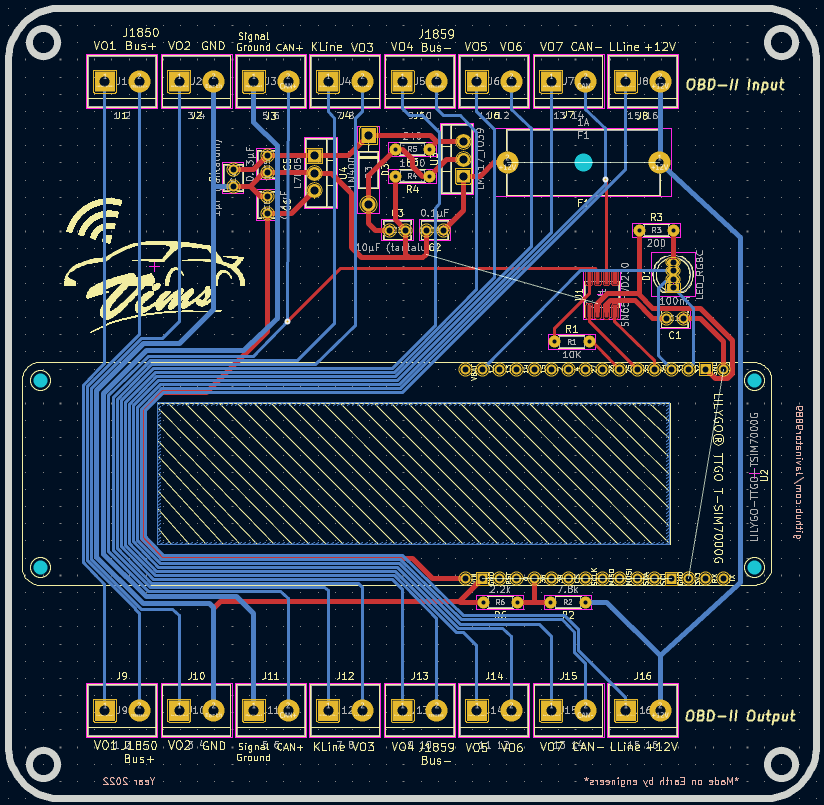
\includegraphics[width=\linewidth]{images/pcb-design.png}
  \caption{Diseño final de la PCB ya enrutada.}
  \label{fig:pcb-design}
\end{figure}

Como se puede apreciar en la figura \ref{fig:pcb-design}, se ha realizado el enrutado
por dos capas. En la capa inferior está principalmente todo el puente entre las
conexiones del \ac{OBD}--II y otros componentes que lo requerían por ubicación. En
la capa superior está enrutado todos los componentes del sistema: reguladores de
tensión, LEDs, transceptor del bus \ac{CAN}, etc. El fusible se encuentra situado
en la esquina superior derecha, justo al lado de la toma de $12V$ del vehículo,
y es quien alimenta a todo el circuito. Si no hay fusible colocado (o se ha fundido)
ningún componente tendrá alimentación. Sin embargo, el puente \ac{OBD}--II seguirá
funcionando.

El renderizado 3D de la PCB sería:

\begin{figure}[H]
  \centering
  \begin{minipage}{.48\linewidth}
    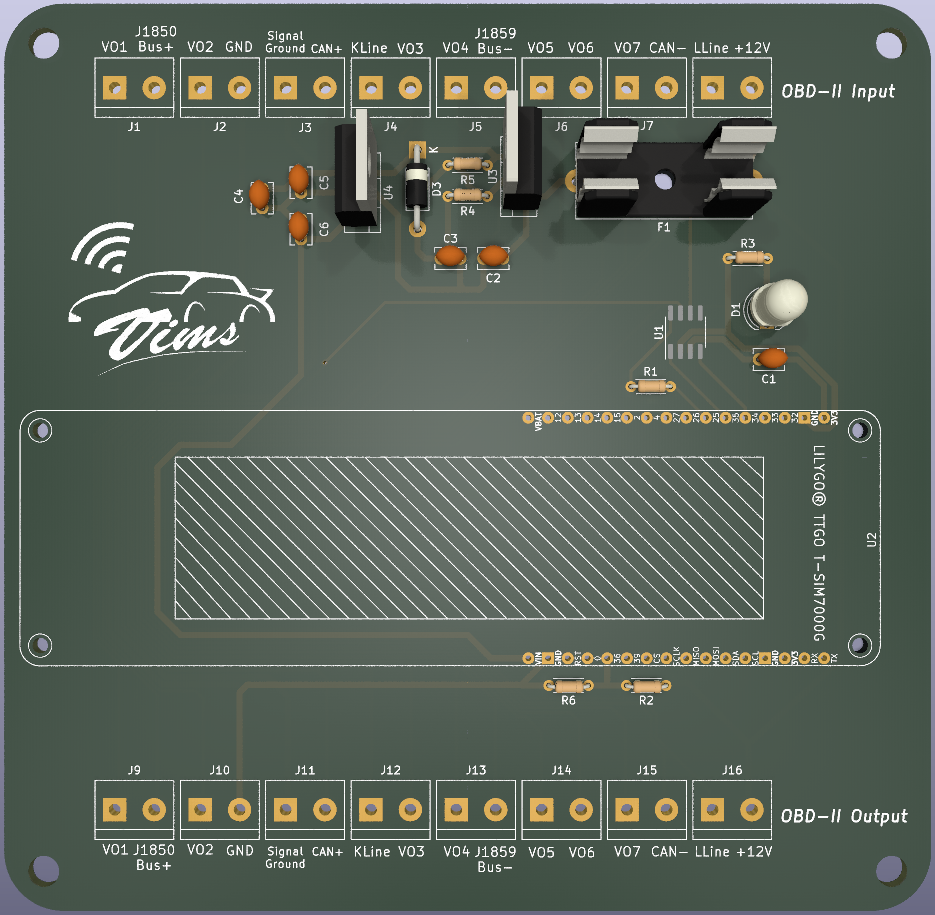
\includegraphics[width=\linewidth]{images/pcb-3d-front.png}
    \caption{Modelo 3D de la placa -- vista posterior.}
    \label{fig:3d-pcb-front}
  \end{minipage}\hfill
  \begin{minipage}{.48\linewidth}
    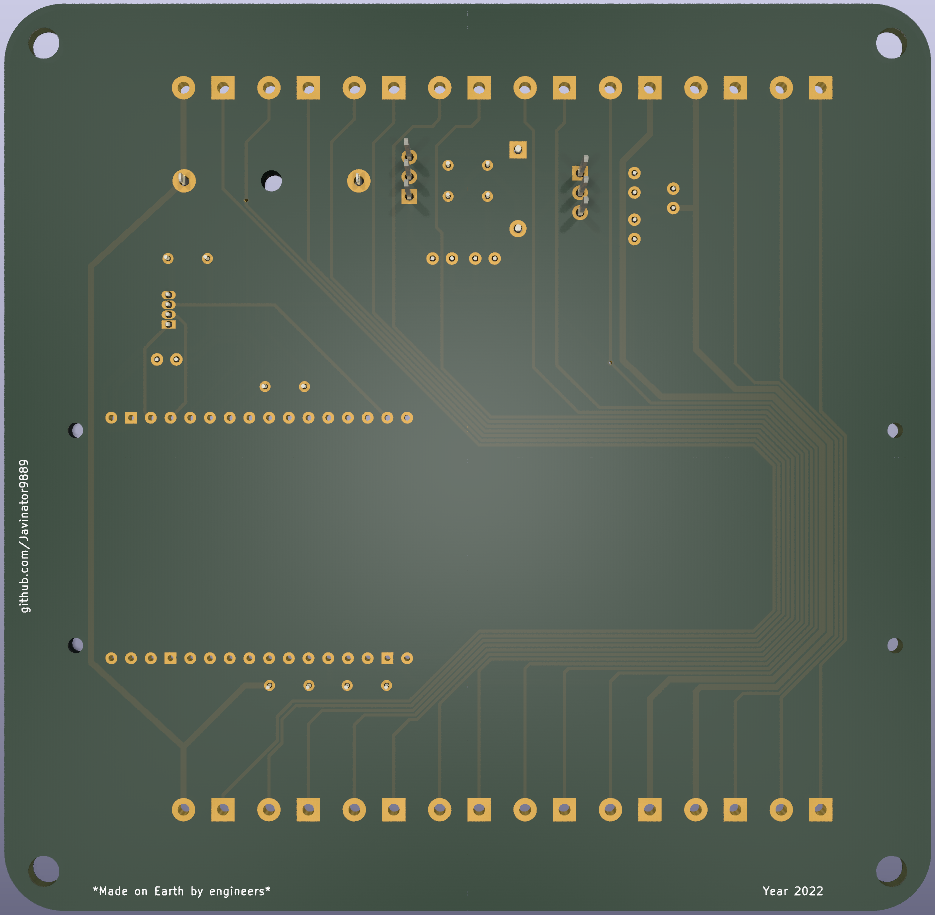
\includegraphics[width=\linewidth]{images/pcb-3d-back.png}
    \caption{Modelo 3D de la placa -- vista anterior.}
    \label{fig:3d-pcb-back}
  \end{minipage}
\end{figure}

Una vez enviadas a fabricar, el resultado que se obtiene es:

\begin{figure}[H]
  \centering
  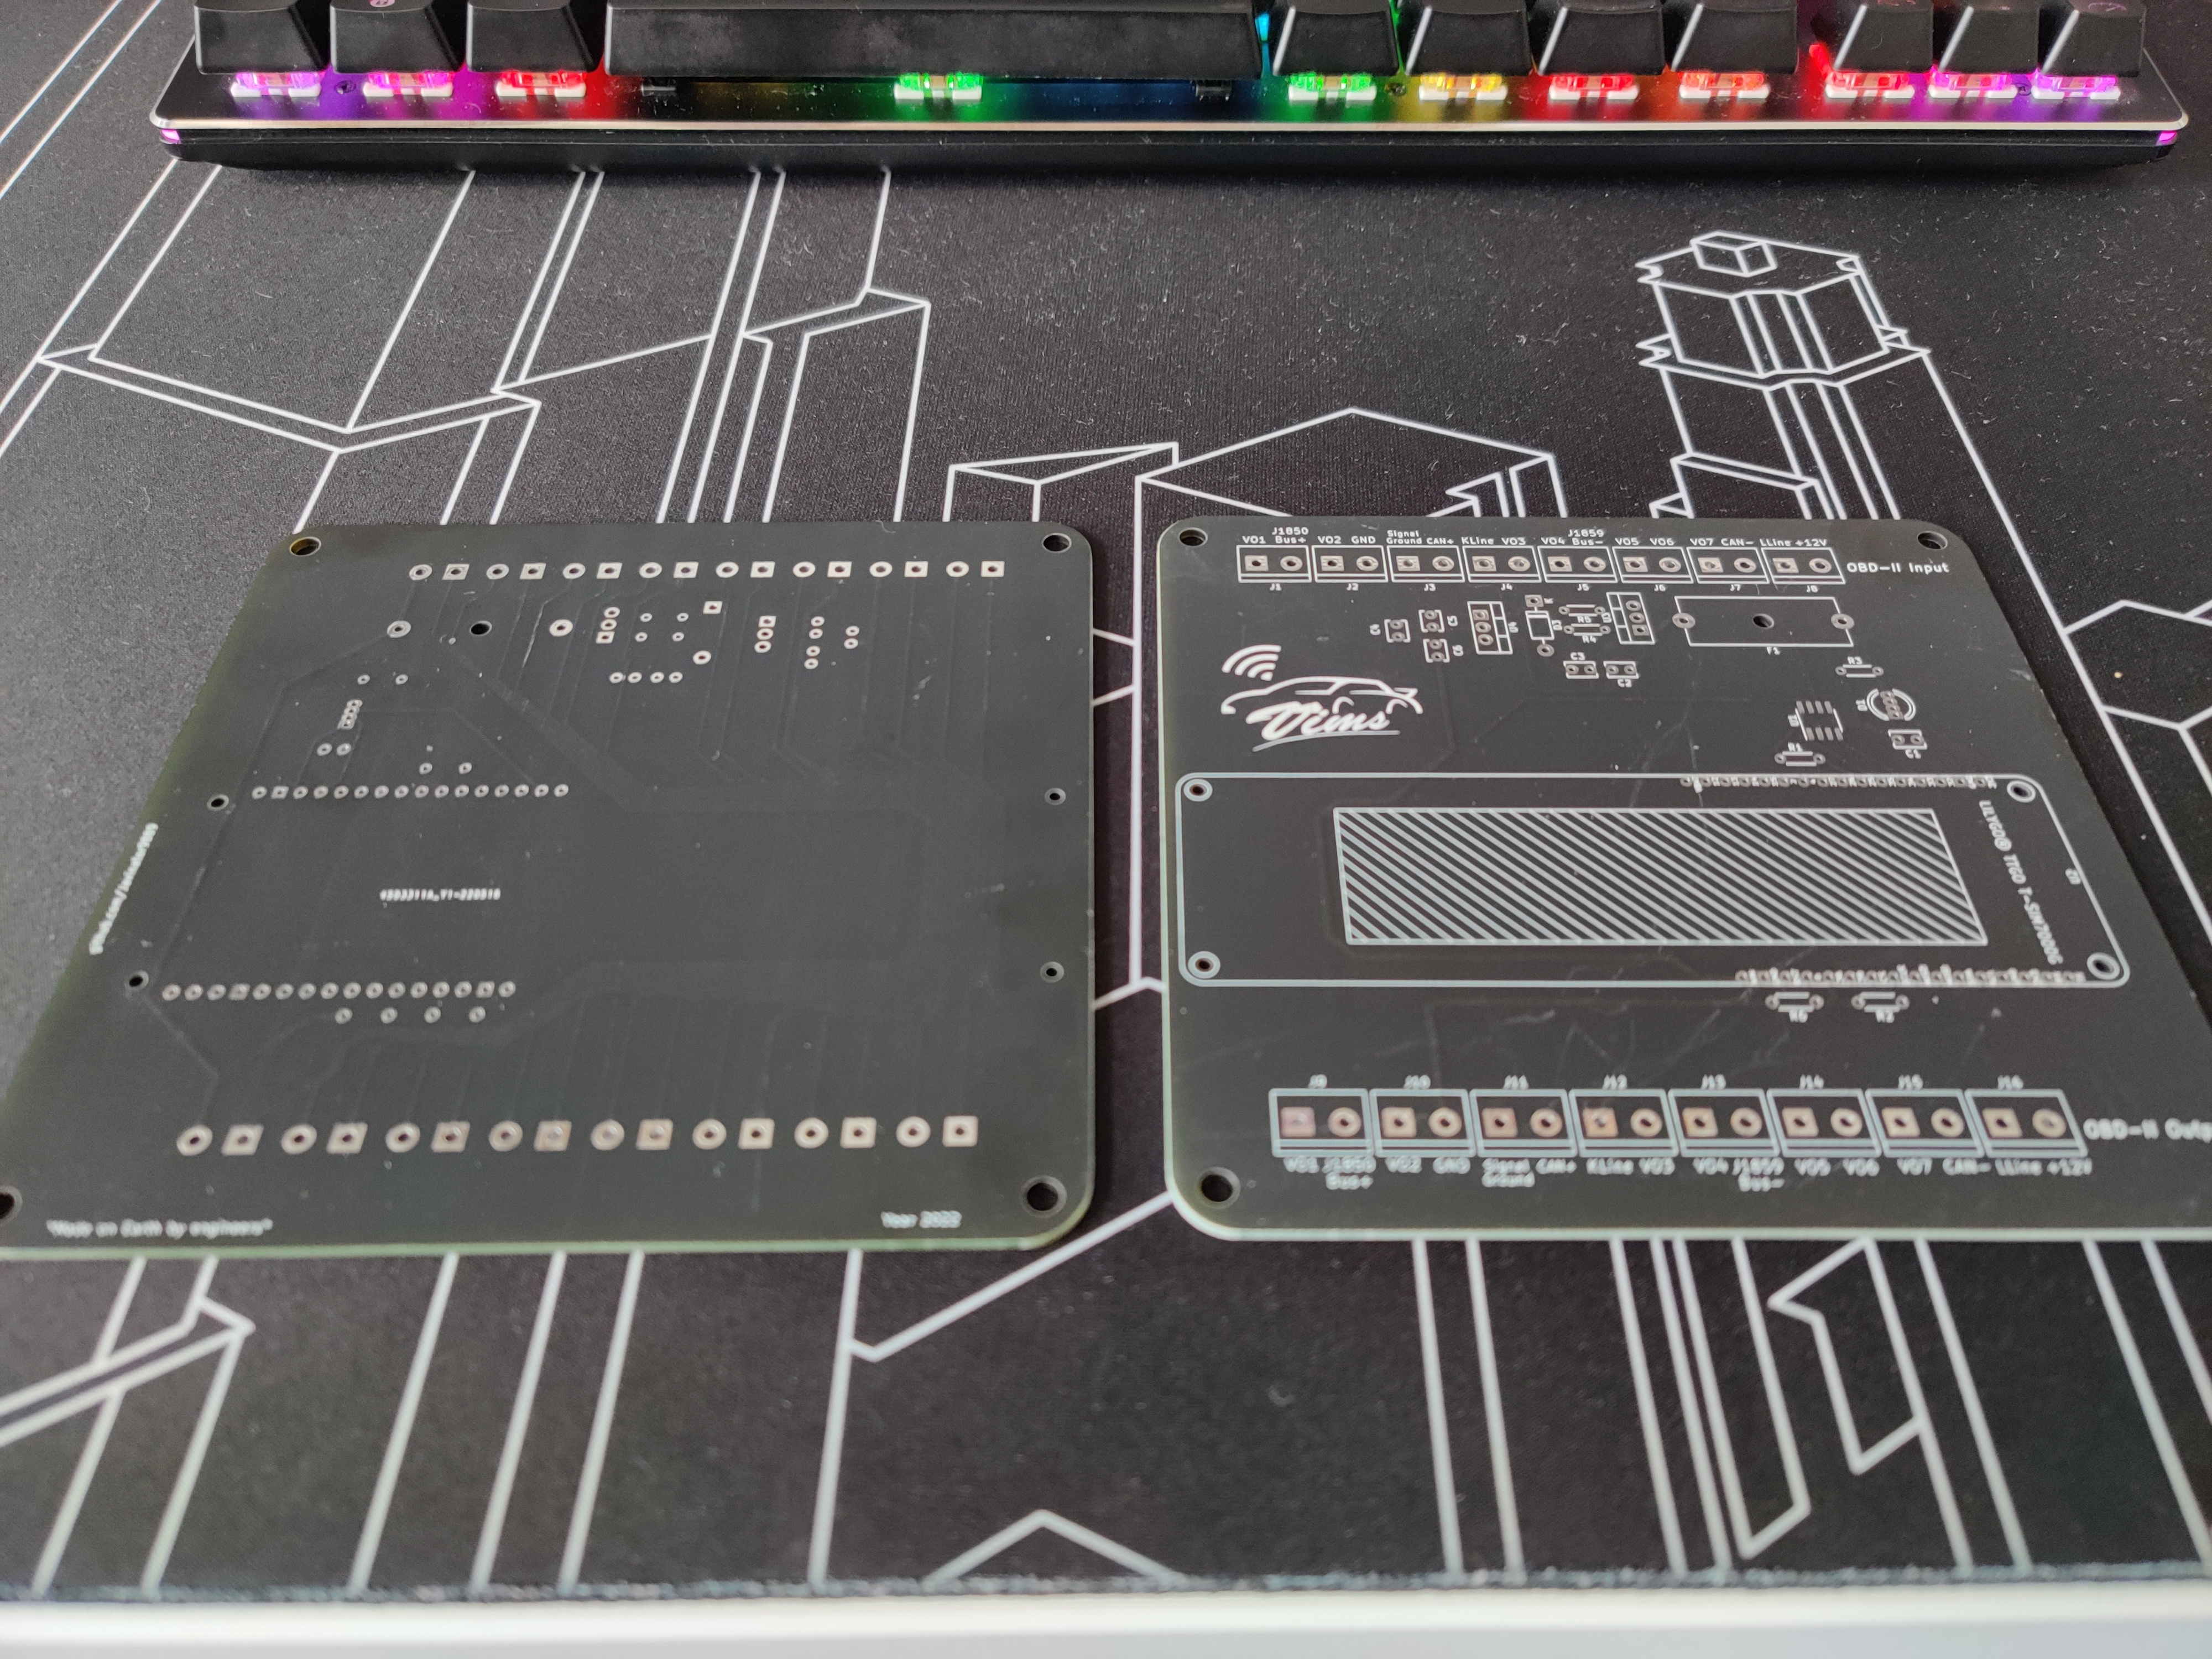
\includegraphics[width=\linewidth]{images/board.jpg}
  \caption{Placa final una vez fabricada.}
  \label{fig:board}
\end{figure}

\begin{figure}[H]
  \centering
  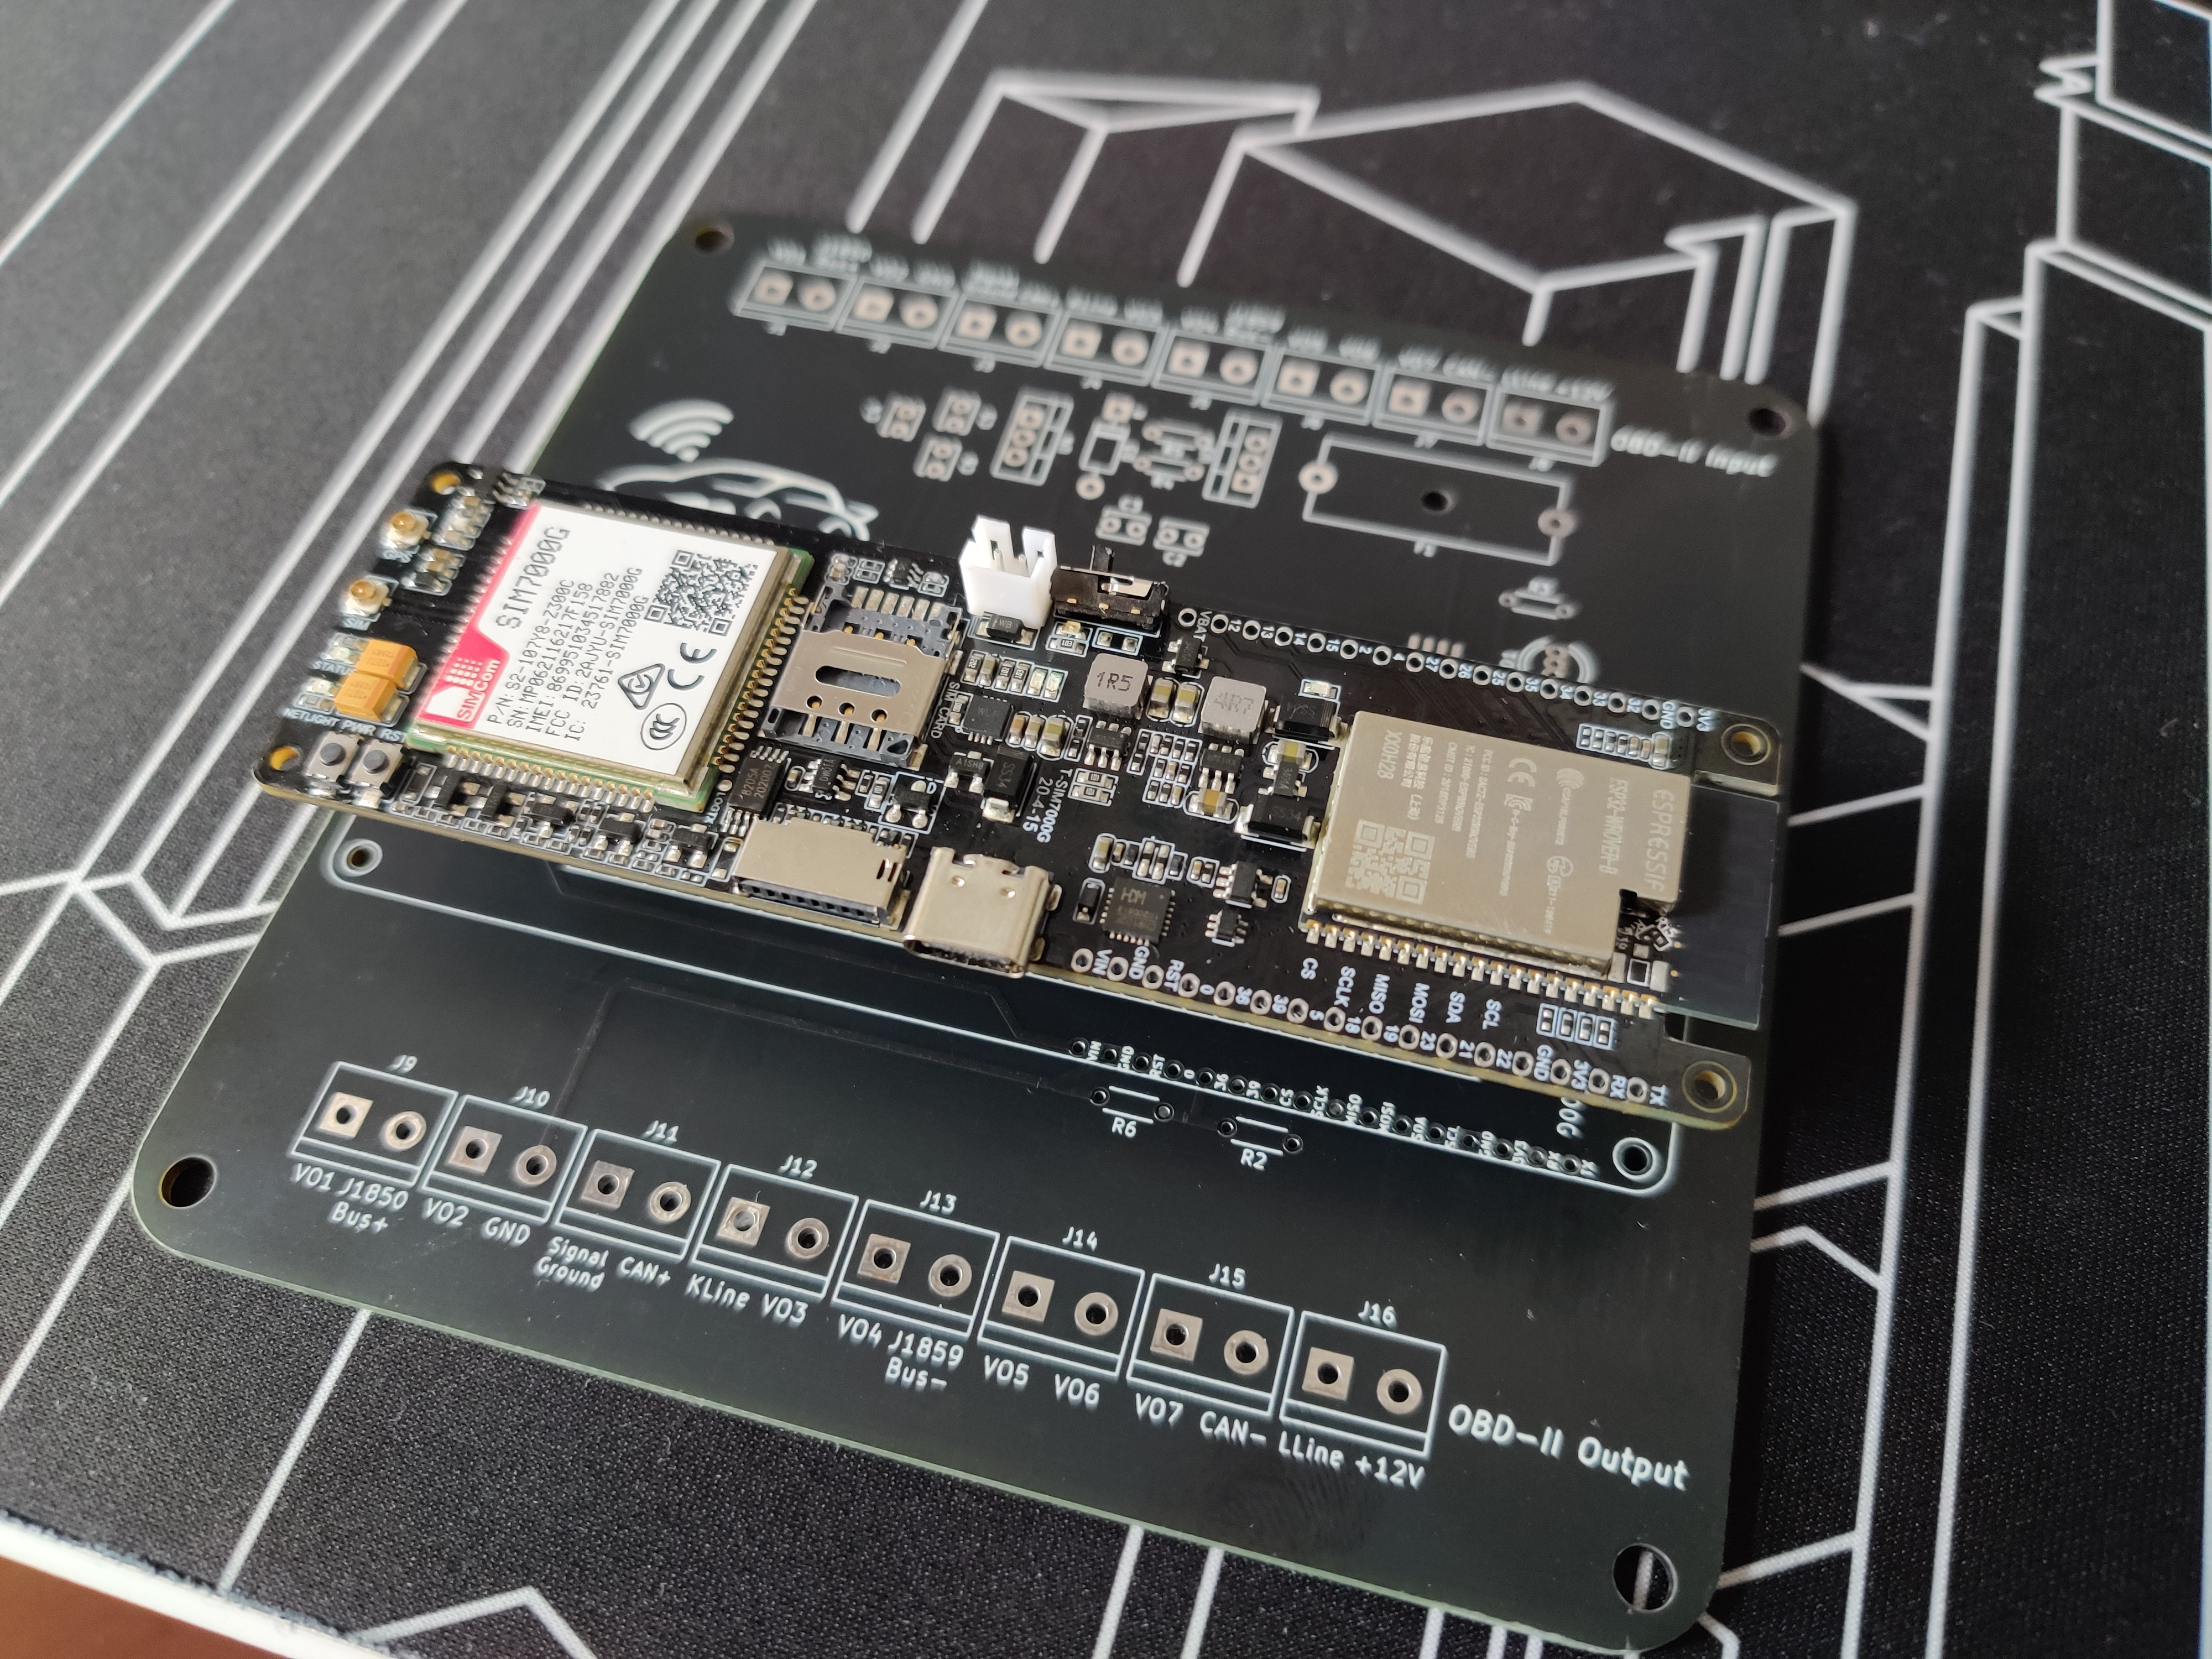
\includegraphics[width=\linewidth]{images/board-with-board.jpg}
  \caption{Visión global de la PCB con la placa T-SIM7000G encima.}
  \label{fig:board-with-board}
\end{figure}
